\documentclass[12pt]{article}
\setlength{\oddsidemargin}{0in}
\setlength{\evensidemargin}{0in}
\setlength{\textwidth}{6.5in}
\setlength{\parindent}{0in}
\setlength{\parskip}{\baselineskip}

\usepackage{amsmath,amsfonts,amssymb,graphicx,enumerate,float}

\begin{document}

CSCI 5454 \hfill Problem Set 4\\
Robert Werthman\\
No Collaborators

\hrulefill

\begin{enumerate}
  \item \textit{Implement the action setting of Hedge and use it to complete a
  few tasks.}
  	\begin{enumerate}
  	  \item \textit{Use Hedge to write a game AI and display some sample output.}
  	    \scriptsize
  	  	\begin{verbatim}
	 	Payoff Matrix
		[-8, 10, 2]
		[-4, -2, -1]
		[-8, -6, 1]
		##########
		Round 0
		##########
		Enter the row you wish to choose: 0
		Action chosen by user 0
		Probability distribution of AI actions [0.3333333333333333,0.3333333333333333,0.3333333333333333]
		Action chosen by AI 1
		AI loss vector [-8, 10, 2]
		AI weight vector [2980.9579870417283, 4.5399929762484854e-05, 0.1353352832366127]
		old AI score 0.0 , new AI score -10.0 , difference -10.0
		old user score 0.0 , new user score 10.0 , difference 10.0
		##########
		Round 1
		##########
		Enter the row you wish to choose: 0
		Action chosen by user 0
		Probability distribution of AI actions [0.9999545869027009, 
		1.522928810416062e-08, 4.5397868011057175e-05]
		Action chosen by AI 0
		AI loss vector [-8, 10, 2]
		AI weight vector [8886110.520507872, 2.061153622438558e-09, 0.018315638888734182]
		old AI score -10.0 , new AI score -2.0 , difference 8.0
		old user score 10.0 , new user score 2.0 , difference -8.0
		##########
		Round 2
		##########
		Enter the row you wish to choose: 0
		Action chosen by user 0
		Probability distribution of AI actions [0.9999999979388461,2.319522825462676e-16,2.0611536181902033e-09]
		Action chosen by AI 0
		AI loss vector [-8, 10, 2]
		AI weight vector [26489122129.84347, 9.357622968840175e-14, 0.002478752176666359]
		old AI score -2.0 , new AI score 6.0 , difference 8.0
		old user score 2.0 , new user score -6.0 , difference -8.0
  		\end{verbatim}
  	  	\normalsize
  	  \item \textit{Give a plot that exhibits $\Theta{(\sqrt{T})}$ regret.}
  	    \begin{figure}[H]
  	    \centering
  	    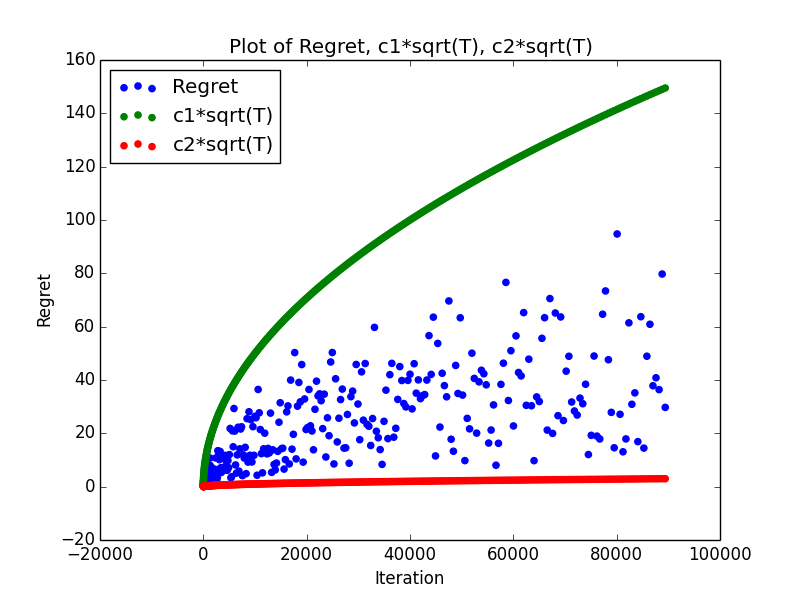
\includegraphics[width=9cm]{q1b.png}
  	    \end{figure}
  	    I let $c_1 = .5$ and $c_2 = .01$ and $\eta = \sqrt{\frac{8ln\,N}{T}}$. 
  	    The graph shows that regret is bounded by $\Theta{(\sqrt{T})}$ where T is the number of rounds. Regret remained
  	    $\le \sqrt(\frac{T}{2}ln\,N)$.  At times regret would get really close to
  	    the bound but other times it would not be close.  It never went above the
  	    bound. Example output of regret in the first column and
  	    $\sqrt(\frac{T}{2}ln\,N)$ in the second column is below.
  	    \scriptsize
  	    \begin{verbatim}
		0.0854754326956 1.16388787282
		0.711207959794 1.55185049709
		0.915738476176 1.93981312136
		1.86659059913 2.32777574563
		1.11868740447 2.7157383699
		0.942107984927 3.10370099418
		1.20108924348 3.49166361845
		2.33209799223 3.87962624272
		2.39799236386 4.26758886699
		3.71141140061 4.65555149126
		3.10138106514 5.04351411554
		1.19507429131 5.43147673981
		3.95892727292 5.81943936408
		0.926603427611 6.20740198835
		2.69832933191 6.59536461262
		0.594289924894 6.9833272369
		6.25916816147 7.37128986117
		3.62512254793 7.75925248544
		0.855690231446 8.14721510971
  	    \end{verbatim}
  	    \normalsize
  	\end{enumerate}
  	
  \newpage
  \item \textit{Show that squared loss guarantees that the best prediction
  in terms of expected loss is going to be x = p.  Give a distribution where
  this is not the case for absolute loss.}\\
  \\
  We want to prove that the expected loss $E[L(x,y)]$ is minimized by letting
  $x=p$.  If $y = 1$ with probability $p$ and $y = 0$ with probability $1-p$
  then 
  \begin{align*}
  E[L(x,y)] &= p \cdot L(x,1) + (1-p) \cdot L(x,0)\\
  &= p \cdot (x-1)^2 + (1-p) \cdot x^2\\
  &= p \cdot (x^2 - 2x + 1) + (1-p)\cdot x^2\\
  &= px^2 - 2px + p + x^2 - px^2\\
  & = x^2 - 2px + p\\
  \end{align*}
  The minimum of a quadratic function of the form $f(x) = ax^2 + bx +c$ can be
  found with the equation 
  $$
  x = -\frac{b}{2a}
  $$
  Solving for $x$ we get 
  $$
  -1 \cdot \frac{(-2px)}{2 \cdot 1} = \frac{2p}{2} = p
  $$
  This shows that the minimum expected loss occurs when is $x=p$.\\
  \\
  Now we want to show that there is a probability distribution for $y=1$ and
  $y=0$ where the expected value of the absolute loss function is not minimized
  when $x=p$.  We can write the expected value of the absolute loss function
  when $y=1,0$ as $$
  E[L(x,y=1,0)] = z|x-1| + w|x-0|
  $$
  where $z$ is the probability of $y=1$ and $w$ is the probability of $y=0$. 
  
  I do not have a solution for this part of the problem.
  
  \newpage
  \item \textit{Use hedge as a subroutine and give an algorithm with will
  always achieve $O(\sqrt{T})$ regret without knowing T ahead of time.}\\
  \\
  \textbf{Pseudocode}\\
  \begin{verbatim}
  def MetaHedge():
    set learning rate to the 1/sqrt(time_horizon_guess).
    start Hedge with inputs time_horizon_guess and learning_rate.
    update the learning rate with a new time_horizon_guess everytime 
    the rounds (T) of the learning algorithm exceed time_horizon_guess. 
  \end{verbatim}
  \textbf{Correctness}\\
  \\
  The solution to this question is using the time horizon guess $\hat{T}$
  to change the learning rate $\eta$ as the algorithm runs in order to keep the
  regret $O(\sqrt{T})$.  Two cases arise with this algorithm when we don't know how many rounds it will run for.
  \begin{enumerate}
    \item The algorithm stops before or at the time horizon guess
    $\hat{T}$.  In this case $\hat{T}$ will be $\ge T$, where $T$ is the
    actual number of rounds the algorithm ran for.  Since we overestimate or
    extimate exactly $T$ with $\hat{T}$, the learning rate $\eta$ and the
    weights and the losses will be as expected or smaller then expected. 
    Because of this when we sum the algorithm loss and the minimum loss of the
    single best predition/action to get regret it will be bounded by
    $O(\sqrt{T})$.
    \item The number of rounds $T$ the algorithm runs for exceeds the time
    horizon guess $\hat{T}$.  An example of this is if we set $\hat{T} = 3$ but
    $T$ ends up running for 4 rounds instead.  In this case once $T=3$ we would
    guess $\hat{T} > 3$ taking us back to the first case above.  We would do
    this over and over again until the algorithm stopped.
  \end{enumerate}
  In both of these cases the regret remains below $\sqrt{T}$ because we
  overestimate the number of rounds $T$ the algorithm runs for with
  time horizon guess $\hat{T}$ which gives us a smaller learning rate $eta$ and
  consistently smaller loss and weight vectors.
  \newpage
  \item \textit{Design an online selling algorithm which will maximize the
  number of customers helped in a hardward store with limited supplies.}
    \begin{enumerate}
      \item \textit{Give a deterministic algorithm with a competitive ratio
      $\le 2$ between the cost of itself and the cost of the optimal offline
      solution like vertex cover.}\\
      \\
      \textbf{Pseudocode}
      \begin{verbatim}
      def OnlineHelpCustomer(customers, store_inventory):
        for each customer:
          for item in customer.set:
            if item in store_inventory:
              return item to sell to customer
          return nothing to sell to customer
      \end{verbatim}
      \textbf{Correctness}\\
      \\
      OnlineCustomerHelp acts like maximal matching.  It chooses
      an item in a customers set and and if that item has not already been
      chosen that item is then sold to that customer.  The customer and item are
      never seen again. In maximal matching the item and customer represent
      vertices and once they have been matched the vertices cannot be used again
      in another match.  For each customer we want to choose an item in their
      set that maximizes the ability of other customers to choose items in
      their sets that have not already been chosen by other customers.\\
      \\
      The difference between the online solution and the optimal offline
      solution is that the offline solution knows all of the items in the sets
      of all the customers.  It can then choose which items are sold to which
      customer to maximize the number of customers who walk away with an item sold to them.\\
      \\
      The offline optimal solution is as follows.  
      \begin{verbatim}
      def OfflineHelpCustomer(customers):
        create a bipartite graph G that contains customers and items
        find the maximal matching in the graph
        sort the customers in descending order by their set size
        start with the customer with the largest set and sell them 
          the item found in the maximal matching
        do this for every customer possible
      \end{verbatim}
      The worst case for either of these aglorithms is when one customer has all
      of the items in their set and the other customers have just one item and that
      item is the same for everyone else.  This leads to the smallest amount of
      customers helped.  For instance if we have two items x and y and customers
      A = \{y,x,z\} , B = \{y\}, C = \{y\}.
      In this case OfflineCustomerHelp would at worst sell two items -- item x
      or z to customer A and then item y to customer B or C.  The
      OnlineCustomerHelp would at worst sell item y because it saw customer
      A first and chose the first item that had not been sold which was y.
      In this case, OnlineHelpCustomer ends up selling one item which is at
      least half of the items sold in OfflineCustomerHelp's solution.\\
      \\
      The cost of the solution to these algorithms is the number of customers
      who don't walk away with an item sold to them.  If you sold $k$ items you
      saw at least $k$ customers which means that if there are $n$ customers
      then $n-k$ customers were not sold an item.
      The pattern for the cost of the solution of OfflineCustomerHelp depends on
      the ceiling of the mean size of the all the customers' sets which indicates
      how many items could be sold.
      The cost of the solution for the online algorithm OnlineCustomerHelp
      depends on the median of the size of all the customer's sets.  The median
      gives the number of items sold to customers.  These patterns for the
      offline and online algorithms give a competitive cost ratio of $$
      OPT/ALG = \frac{n-mean(|S_n|)}{n-median(|S_n|)}
      \le 2.
      $$

      \item \textit{Show that every deterministic algorithm has competitive
      ratio $\le 2$.}\\
      \\
      \textbf{Problem Statement}\\
      \\
      ALG is the cost found by a deterministic algorithm for a solution and
      OPT is the cost of the optimal solution.  OPT will give the minimized cost
      to the solution. In order for every deterministic algorithm to have a
      competitive ratio of at least 2 we have to assume that $$
      OPT/ALG \le 2
      $$
      \textbf{Proof}\\
      \\
      We know that the cost of a solution given by a deterministic algorithm
      will be either greater or the same as the cost of the optimal solution. 
      This gives us the inequality
      $$
      OPT \le ALG
      $$
      In fact the cost of the solution given by a deterministic algorithm could
      be any constant $c$, $c \ge 1$, times the optimal
      solution.
      This produces the inequality
      $$
      OPT \le c \cdot ALG
      $$
      This says that the OPT will produce a cost less than or equal to the cost
      produced by the deterministic algorithm.  If we let $c=2$ than
      $$
      OPT/ALG \le 2
      $$
      \item \textit{Prove that the expected value of the competitive ratio of
      randomized version of the online selling algorithm is $< 2$.}\\
      \\
      If customer $i$ arrives at the shop and wishes to purchase an item, the
      probability of them receiving any item from their set is 
      $$
      p_i = \frac{1}{S_i \cup U_i}
      $$
      If $X$ is the random variable that represents the number of customers
      that receive an item from the store, the expected value of all $n$
      customers receiving an item is 
      $$ 
      E[X] = \sum_{i=1}^{n} i \cdot p_i = \sum_{i=1}^{n} i \cdot \frac{1}{S_i
      \cup U_i} $$
      The cost of the randomized version of the online selling algorithm is then
      equal to
      $$
      n - E[X]
      $$
      which is the number of customers that do not receive an item.\\
      \\
      We want to show that the competitive ratio of the expectation of this
      randomized algorithm is less than 2 as shown in the equation below 
      $$
      \frac{OPT}{ALG} < 2 \Longrightarrow \frac{OPT}{n-E[X]} < 2
      $$
      From 4a, we said $OPT = n-mean(|S_n|)$ which means the cost of the optimal
      solution is equal to the total number of customers $n$ minus the average
      number of items in the customers' sets.  This makes the equation above
      $$
      \frac{OPT}{ALG} = \frac{n-mean(|S_n|)}{n-E[X]} < 2
      $$
      Because you can say the $E[X]$ is the average of the random variable $X$,
      if we have $n$ customers than we can expect $n/2$ customers to receive an item.  This simplifies
      our competitive ratio equation to 
      $$
      \frac{n-mean(|S_n|)}{n-E[X]} = \frac{n-mean(|S_n|)}{n-n/2} =
      \frac{n-mean(|S_n|)}{n/2} < 2 
      $$
      Furthermore the averge number of items in the customers' sets
      $mean(|S_i|)$ will be $\ge 1$ (all customers have only one item in their
      set) and $\le n$ (all customers have all the items in their set).
      This gives us two boundaries to test for the competitive ratio.  Setting $mean(|S_n|) = n$ the competive ratio holds.
      $$
      \frac{n-n}{n/2} = 0 < 2
      $$
      Setting $mean(|S_n|) = 1$ the competitve ratio also holds.
      $$
      \frac{n-1}{n/2} = \frac{2n-2}{n} < 2
      $$
      If we take the limit of $\frac{2n-2}{n}$ in regards to $n$, it approaches
      2 so we can say that 
      $$
      \frac{2n-2}{n} < 2.
      $$
      \\Because the competitive ratio holds for both these cases the
      competitive ratio of the expection of the cost of the randomized algorithm
      for online selling is $< 2$.
    \end{enumerate}
    
  \newpage
  \item \textit{Find a mixed nash equilibrium of the zero-sum game.  Give both
  strategies and the value of the game and show the vector of expected payoffs
  for player 2 under player 1's strategy and vice versa.}
    $$
    M = \begin{bmatrix}
        1 & 0 & 1 & 8 & 0\\
        5 & 8 & 9 & 2 & 1\\
        0 & 1 & 8 & 0 & 5\\
        8 & 9 & 2 & 1 & 0\\
        1 & 8 & 0 & 5 & 8\\
        \end{bmatrix}
    $$
  A mixed nash equilibrium means that player 1 and player 2 won't want to
  deviate from strategies that they choose and those strategies will lead to the same
  value of the game.  Those strategies are based on probabilities for each
  decision they can make. The row player wants to minimize the value in the
  row he chooses from the matrix and the column player wants to
  maximize the value in the column he chooses from the matrix.\\
  \\
  I used hedge to find the mixed nash equilibrium.  The strategy for the row
  player was the row distribution after 25 rounds of hedge [[  9.99985259e-01  
  6.52573142e-07 1.34647736e-05   6.23766866e-07 4.42372909e-11]].  The row
  payoff was [[ 25.43045603][ 25.43045603][ 25.43045603][25.43045603][ 25.43045603]] for each row.\\
  \\ 
  The strategy for the column player was the column distribution [[ 
  4.67085924e-02] [  2.39700681e-01] [  2.90734717e-03][  3.45778443e-13][  7.10683379e-01]].  
  The column payoff vector ended up being [[-25.43045603 -25.43045603
  -25.43045603 -25.43045603 -25.43045603]].\\
  \\
  The value for the game approached 0.0019868 which was the time-averaged
  expected payoff of both the row and column players.  As you can see the sum
  of the row and column payoff vectors equals 0 resulting in a zero-sum game.
  
  A sample run of two rounds from my program is below.
  \scriptsize
  \begin{verbatim}
  ##########
Round 0
##########
row distribution [[ 0.2  0.2  0.2  0.2  0.2]]
column distribution [[ 0.2]
 [ 0.2]
 [ 0.2]
 [ 0.2]
 [ 0.2]]
row payoff [[ 3.64]
 [ 3.64]
 [ 3.64]
 [ 3.64]
 [ 3.64]]
column payoff [[-3.64 -3.64 -3.64 -3.64 -3.64]]
row loss [[ 2. ]
 [ 5. ]
 [ 2.8]
 [ 4. ]
 [ 4.4]]
column loss [[ 3.   5.2  4.   3.2  2.8]]
##########
Round 1
##########
row distribution [[ 0.27099839  0.14872707  0.23092959  0.18165565  0.1676893 ]]
column distribution [[ 0.2239959 ]
 [ 0.14426152]
 [ 0.18339233]
 [ 0.2152129 ]
 [ 0.23313735]]
row payoff [[ 6.93206598]
 [ 6.93206598]
 [ 6.93206598]
 [ 6.93206598]
 [ 6.93206598]]
column payoff [[-6.93206598 -6.93206598 -6.93206598 -6.93206598 -6.93206598]]
row loss [[ 2.12909141]
 [ 4.58816581]
 [ 2.77708693]
 [ 3.67231845]
 [ 4.31925133]]
column loss [[ 2.63556824  4.39716141  3.82029004  3.48554339  2.64488944]]
  \end{verbatim}
  \normalsize
    
\end{enumerate}


\end{document}